% Provenance (never printed): old seconde/premiere S material on water as a
% resource (stocks and flows of the water cycle, residence times, groundwater,
% overuse as a physical fact); see sources/book2/PROVENANCE.md. Residence
% times are computed in figdata/grade-10/residence_times.py, the Aral Sea
% budget in figdata/grade-10/aral_sea.py.
\chapter{Zoetwatervoorraden}\label{ch:g10:freshwater-resources}

In 1960 was het Aralmeer, in de woestijnen van Centraal-Azië, het op drie na
grootste meer ter wereld. Twee grote rivieren, gevoed door sneeuw en regen in
verre bergen, stroomden erin; geen enkele stroomde eruit. In de jaren 1960 werd
hun water afgetapt om de woestijn te irrigeren. Satellieten hebben gezien wat er
volgde: het meer is in stukken uiteengevallen, en het grootste deel van de bodem
is nu droog land. De oorzaak was verreweg niet een verandering van het klimaat,
maar de irrigatie: het meer kreeg elk jaar veel minder water dan de verdamping
eraan onttrok. Dit hoofdstuk telt het water van de Aarde, waar het is opgeslagen
en hoe snel het beweegt, en laat zien dat een watervoorraad vooral een stroom is:
wanneer er meer uit een reservoir wordt gehaald dan erin stroomt, loopt het
reservoir leeg, in een tempo dat een eenvoudige balans voorspelt.
% ledger: nasa:aral, gaybullaev:aral-1960, micklin:aral

\begin{omfigure}
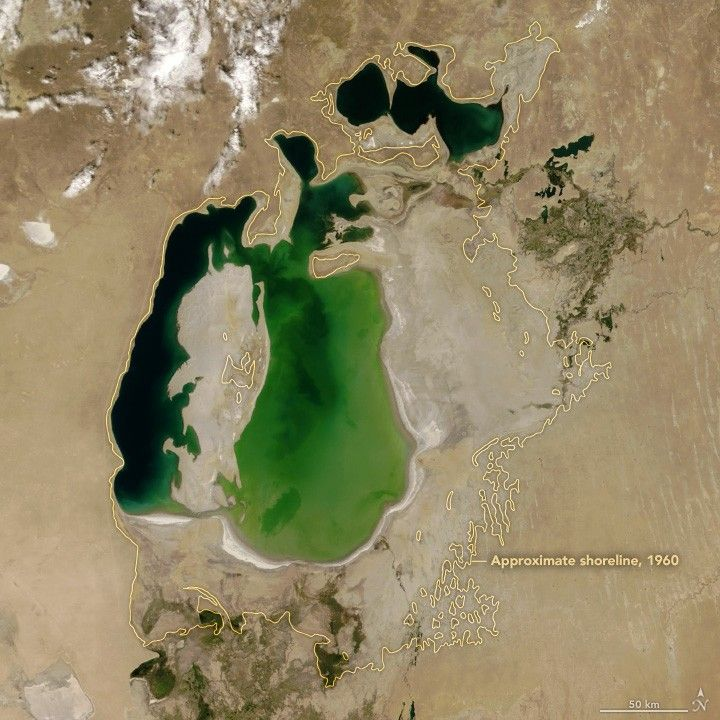
\includegraphics[width=0.47\linewidth]{images/book2/g10-nasa-aral-2000.jpg}\hspace{0.03\linewidth}%
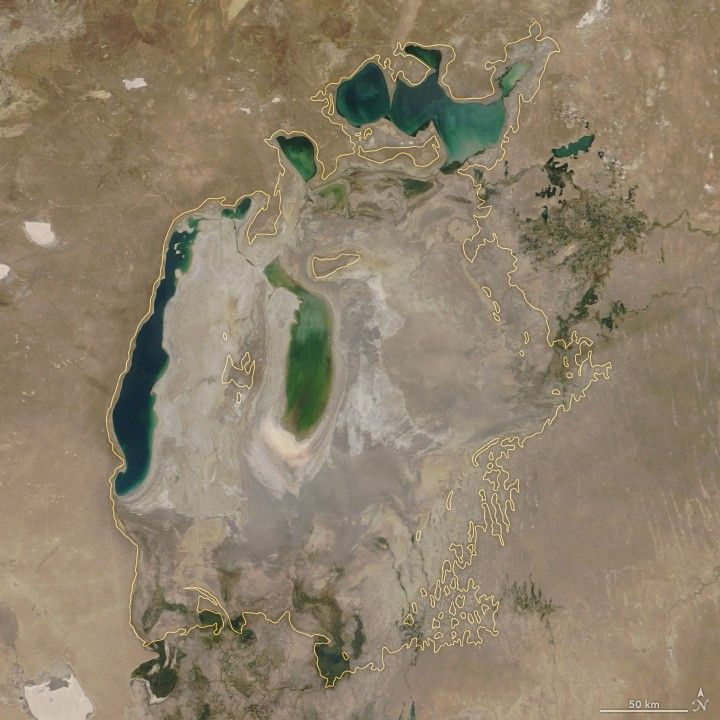
\includegraphics[width=0.47\linewidth]{images/book2/g10-nasa-aral-2018.jpg}

{\small Het Aralmeer gezien door het MODIS-instrument van NASA's Terra-satelliet
in augustus 2000 (links) en augustus 2018 (rechts); de gele lijn is bij benadering
de oever van 1960. De schaalstreep is \qty{50}{km}. Beelden: NASA Earth
Observatory.}
\end{omfigure}

\begin{recall}
De waterkringloop verplaatst water tussen de oceaan, de lucht en het land:
verdamping, condensatie tot wolken, neerslag, afstroming; de totale massa water
blijft behouden (de natuurkundeboeken). Gesteenten met verbonden poriën zijn
doorlatend; onder de grondwaterspiegel zijn hun poriën vol water, en een laag die
genoeg water bevat en doorlaat om putten te voeden, is een watervoerende laag
(Boek 1, jaar 6). Het meeste water van de Aarde is zout water (Boek 1,
jaar 2). Een rivier voert het water van haar \omterm{def:g10:drainage-basins:drainage-basin}{stroomgebied} af; haar \omterm{def:g10:drainage-basins:discharge}{afvoer} is een
volume per seconde (\cref{ch:g10:drainage-basins}).
\end{recall}

\section{Waar het water is}

De Aarde bevat ongeveer 1.39 miljard kubieke kilometer water. Bijna alles daarvan
zit in de oceaan; maar \qty{2.5}{\percent} is zoet. En het meeste van dat zoete
water is onbereikbaar: meer dan twee derde ervan is bevroren in de ijskappen en
gletsjers, en bijna een derde zit onder de grond.
% ledger: usgs:water-stocks

\begin{center}
\small
\begin{tabular}{|l|r|r|}
\hline
\textbf{reservoir} & \textbf{volume (\unit{km^3})} & \textbf{aandeel van het zoete water} \\ \hline
oceanen, zeeën en baaien & \num{1338000000} & (zout) \\ \hline
ijskappen, gletsjers en eeuwige sneeuw & \num{24064000} & \qty{68.7}{\percent} \\ \hline
zoet grondwater & \num{10530000} & \qty{30.1}{\percent} \\ \hline
grondijs en permafrost & \num{300000} & \qty{0.86}{\percent} \\ \hline
zoetwatermeren & \num{91000} & \qty{0.26}{\percent} \\ \hline
bodemvocht & \num{16500} & \qty{0.05}{\percent} \\ \hline
atmosfeer & \num{12900} & \qty{0.04}{\percent} \\ \hline
rivieren & \num{2120} & \qty{0.006}{\percent} \\ \hline
\end{tabular}

{\small Eén schatting van het water van de wereld, naar Shiklomanov (1993), via de
U.S. Geological Survey. Zout grondwater (\num{12870000}~\unit{km^3}) en
zoutmeren zijn weggelaten.}
\end{center}
% ledger: usgs:water-stocks

Rivieren en zoetwatermeren, waaruit mensen het meeste water halen dat ze
gebruiken, bevatten samen minder dan een honderdste procent van al het water.
Toch staan rivieren nooit lang droog: ze zijn geen \omterm{def:g10:freshwater-resources:stock}{voorraad} maar een stroom, die
door elke regenbui wordt aangevuld.

\section{Voorraden en fluxen}

\begin{definition}[Voorraad; flux]\label{def:g10:freshwater-resources:stock}
In een waterbalans is een \emph{voorraad}\index{voorraad (van water)} de
hoeveelheid water die op een bepaald moment in een reservoir zit --- de oceaan,
de lucht, het ijs, een watervoerende laag, een meer ---, als volume of als massa.
Een \emph{flux}\index{flux (van water)} is de hoeveelheid die per tijdseenheid
van het ene reservoir naar het andere gaat, bijvoorbeeld in kubieke kilometer per
jaar.
\end{definition}

Een \omterm{def:g10:freshwater-resources:stock}{voorraad} verandert alleen door zijn \omterm{def:g10:freshwater-resources:stock}{fluxen}: wat erin komt min wat eruit gaat.
Als die twee gelijk zijn, is de \omterm{def:g10:freshwater-resources:stock}{voorraad} in een \emph{stationaire toestand}: hij
blijft gelijk, hoewel zijn water voortdurend wordt vervangen.

\begin{omfigure}
\begin{tikzpicture}[font=\footnotesize, >={Stealth[length=6pt]}]
  % ocean, land, atmosphere
  \fill[omSea] (0,0) rectangle (6.4,1.6);
  \fill[omLithAlluv] (6.4,0) -- (6.4,1.6) -- (8.2,2.1) -- (10.4,2.6) -- (12,2.9) -- (12,0) -- cycle;
  \fill[omLithSand!60] (6.4,0) -- (12,0) -- (12,1.0) -- (6.4,0.7) -- cycle;
  \draw[black!50] (6.4,1.6) -- (8.2,2.1) -- (10.4,2.6) -- (12,2.9);
  \fill[omIce] (10.6,2.65) -- (11.3,3.35) -- (12,2.9) -- cycle;
  \node[align=center] at (3.2,0.75) {\textbf{oceaan}\\\num{1335040}};
  \node[align=center] at (9.3,1.35) {bodemvocht 122\\meren en rivieren 178};
  \node[align=center] at (9.3,0.35) {grondwater \num{15300}};
  \node[align=center] at (11.2,2.25) {ijs\\\num{26350}};
  % atmosphere
  \draw[black!30, rounded corners=8pt, fill=omWxCloud] (1.0,4.6) rectangle (11.0,5.6);
  \node[align=center] at (6.0,5.1) {\textbf{atmosfeer} 12.7};
  % fluxes
  \draw[->, omProp, line width=1.4pt] (1.4,1.7) -- node[left, align=right] {verdamping\\413} (1.4,4.5);
  \draw[->, omWxRain, line width=1.4pt] (4.4,4.5) -- node[pos=0.3, right, align=left] {neerslag\\373} (4.4,1.7);
  \draw[->, omWxRain, line width=1.4pt] (7.6,4.5) -- node[pos=0.7, left, align=right] {neerslag\\113} (7.6,2.05);
  \draw[->, omProp, line width=1.4pt] (10.0,2.6) -- node[right, align=left] {verdamping en\\transpiratie 73} (10.0,4.5);
  \draw[->, black!60, line width=1.2pt] (4.9,5.85) -- node[above] {waterdamp over het land gevoerd: 40} (7.4,5.85);
  \draw[->, omRiver, line width=1.4pt] (7.6,1.2) -- node[above, inner sep=2pt] {afstroming 40} (6.0,1.2);
\end{tikzpicture}

{\small De wereldwijde waterkringloop van de jaren 1990 (schematisch; niet op
schaal). Voorraden in duizenden \unit{km^3}, \omterm{def:g10:freshwater-resources:stock}{fluxen} in duizenden \unit{km^3} per
jaar. Naar Trenberth en anderen (2007). Schattingen van de voorraden verschillen
van studie tot studie: vergelijk het grondwater en het ijs hier met de tabel
hierboven.}
\end{omfigure}
% ledger: trenberth:water-cycle

De kringloop is in evenwicht. Elk jaar verliest de oceaan \num{413000}~\unit{km^3}
door verdamping en krijgt hij \num{373000} terug als regen en sneeuw en
\num{40000} uit de rivieren. De lucht ontvangt $413\,000 + 73\,000 = \num{486000}$~\unit{km^3}
en geeft $373\,000 + 113\,000$ terug, evenveel. Het land ontvangt
\num{113000}~\unit{km^3} neerslag; \num{73000} keren terug naar de lucht door
verdamping en via de bladeren van planten, en de overige \num{40000} stromen af
naar zee, in rivieren en ondergronds.
% ledger: trenberth:water-cycle

\begin{definition}[Hernieuwbaar zoet water]\label{def:g10:freshwater-resources:renewable}
Het \emph{hernieuwbare zoete water}\index{hernieuwbaar zoet water} van een gebied
is de \omterm{def:g10:freshwater-resources:stock}{flux} zoet water die elk jaar door neerslag wordt vernieuwd en die er als
afstroming in rivieren en als grondwater doorheen stroomt. Het is een \omterm{def:g10:freshwater-resources:stock}{flux}, in
kubieke kilometer per jaar, geen \omterm{def:g10:freshwater-resources:stock}{voorraad}.
\end{definition}

Voor al het land van de Aarde is het de \num{40000}~\unit{km^3} die elk jaar de
zee bereikt. Een gebied kan zijn hernieuwbare water jaar na jaar gebruiken zonder
tekort te komen. Wat het daarbovenop neemt, kan alleen uit een \omterm{def:g10:freshwater-resources:stock}{voorraad} komen,
die dan krimpt.

\section{Verblijftijd}

Hoe lang blijft een watermolecuul in een reservoir? Sommige gaan er meteen weer
uit, andere blijven veel langer; maar gemiddeld volgt het antwoord uit de
\omterm{def:g10:freshwater-resources:stock}{voorraad} en de \omterm{def:g10:freshwater-resources:stock}{flux} alleen.

\begin{definition}[Verblijftijd]\label{def:g10:freshwater-resources:residence-time}
De \emph{verblijftijd}\index{verblijftijd} van water in een reservoir is de
gemiddelde tijd die water er doorbrengt tussen binnenkomen en weggaan.
\end{definition}

\begin{proposition}[Verblijftijd, voorraad en flux]\label{prop:g10:freshwater-resources:residence}
Voor een reservoir in stationaire toestand, met een \omterm{def:g10:freshwater-resources:stock}{voorraad} $S$ waar een \omterm{def:g10:freshwater-resources:stock}{flux} $F$
doorheen gaat (erin en eruit), is de \omterm{def:g10:freshwater-resources:residence-time}{verblijftijd}
\[
T = \frac{S}{F}.
\]
\end{proposition}

\begin{proof}
In stationaire toestand komt er elk jaar een volume $F$ in en gaat er een volume
$F$ uit, terwijl de \omterm{def:g10:freshwater-resources:stock}{voorraad} $S$ blijft. Na een tijd $S/F$ is er een volume
$F \times S/F = S$ binnengekomen: evenveel als het hele reservoir bevat.
Gemiddeld is het water dat er aan het begin was dan vervangen, dus blijft het
water $S/F$ in het reservoir.
\end{proof}

\begin{example}[Water in de lucht]\label{ex:g10:freshwater-resources:atmosphere}
De atmosfeer bevat \num{12700}~\unit{km^3} water, en er valt elk jaar
\num{486000}~\unit{km^3} uit als regen en sneeuw. De \omterm{def:g10:freshwater-resources:residence-time}{verblijftijd} is
$12\,700/486\,000 \approx \num{0.026}$ jaar, ongeveer \num{9.5} dagen: het
water van de lucht wordt elke week of twee weken vernieuwd. Een wolk die vandaag
regent, bestaat uit water dat een paar dagen geleden de oceaan of de grond
verliet.
\end{example}
% ledger: trenberth:water-cycle (t_atmosphere_days 9.5 in figdata/grade-10/residence_times.py)

Dezelfde berekening geeft ongeveer \num{19} dagen voor het water in de
rivierbeddingen ($2120$~\unit{km^3} afgevoerd met \num{40000}~\unit{km^3} per
jaar), een paar jaar voor meren en rivieren samen, en ongeveer \num{3200} jaar
voor de oceaan ($1\,335\,040/413$ duizend~\unit{km^3}). Grondwater kan nog trager
zijn: het diepste water van sommige watervoerende lagen is honderdduizenden jaren
oud.
% ledger: trenberth:water-cycle, usgs:water-stocks, sturchio:nubian-age

\begin{omfigure}
\begin{tikzpicture}
\begin{axis}[omrecord, xbar, xmode=log, log origin=infty, width=0.74\linewidth, height=5.6cm,
  xmin=1, xmax=1e9, ymin=-0.6, ymax=4.6, bar width=11pt,
  ytick={0,1,2,3,4}, yticklabels={atmosfeer, rivieren, {meren en rivieren}, oceaan, {diep grondwater (ouderdom)}},
  xtick={1,30.44,365.25,36525,3652500,365250000}, xticklabels={1 dag, 1 maand, 1 jaar, 100 jaar, \num{10000} jaar, 1 miljoen jaar},
  xticklabel style={font=\scriptsize, rotate=25, anchor=north east}, yticklabel style={font=\small},
  xlabel={verblijftijd (logaritmische schaal)}, label style={font=\small}, xmajorgrids]
\addplot[fill=omDef!45, draw=omDef!80!black] table[x=days, y=idx] {figdata/out/grade-10-residence_times-times.dat};
\draw[fill=omProp!45, draw=omProp!80!black] (axis cs:73050000,3.75) rectangle (axis cs:365250000,4.25);
\node[anchor=west, font=\scriptsize] at (axis cs:9.5,0) {\num{9.5} dagen};
\node[anchor=west, font=\scriptsize] at (axis cs:19.4,1) {\num{19} dagen};
\node[anchor=west, font=\scriptsize] at (axis cs:1625,2) {\num{4.5} jaar};
\node[anchor=west, font=\scriptsize] at (axis cs:1180690,3) {\num{3200} jaar};
\node[anchor=east, font=\scriptsize] at (axis cs:73050000,4) {\num{200000} tot 1 miljoen jaar};
\end{axis}
\end{tikzpicture}

{\small \omterm{def:g10:freshwater-resources:residence-time}{Verblijftijden} van water, berekend als \omterm{def:g10:freshwater-resources:stock}{voorraad} gedeeld door \omterm{def:g10:freshwater-resources:stock}{flux} uit de
wereldwijde waterkringloop (blauw), en de gemeten ouderdom van diep grondwater
onder de oostelijke Sahara (oranje). Logaritmische as: vanaf één jaar is elke
gemarkeerde stap een factor honderd. Gegevens: Trenberth en anderen (2007); U.S.
Geological Survey; Sturchio en anderen (2004).}
\end{omfigure}
% values computed in figdata/grade-10/residence_times.py

De \omterm{def:g10:freshwater-resources:residence-time}{verblijftijd} meet hoe snel een reservoir zich herstelt. Water dat uit een
rivier wordt gehaald, is in enkele dagen vervangen; een vervuild of leeggemaakt
meer heeft jaren nodig; grondwater waarvan het verzamelen duizenden jaren duurde,
wordt op de schaal van een mensenleven helemaal niet vernieuwd.

\begin{method}[Een waterbalans]\label{met:g10:freshwater-resources:budget}
\begin{enumerate}
  \item Kies het reservoir: een meer, een watervoerende laag, een \omterm{def:g10:drainage-basins:drainage-basin}{stroomgebied}, de lucht.
  \item Maak een lijst van elke \omterm{def:g10:freshwater-resources:stock}{flux} erin (rivieren, regen, insijpeling) en eruit
        (rivieren, verdamping, oppompen), in dezelfde eenheid.
  \item De verandering van de \omterm{def:g10:freshwater-resources:stock}{voorraad} per jaar is de som van de inkomsten min de
        som van de uitgaven.
  \item Als de \omterm{def:g10:freshwater-resources:stock}{voorraad} niet verandert, zijn de inkomsten gelijk aan de uitgaven,
        en is de \omterm{def:g10:freshwater-resources:residence-time}{verblijftijd} de \omterm{def:g10:freshwater-resources:stock}{voorraad} gedeeld door een van beide.
\end{enumerate}
\end{method}

\section{Watervoerende lagen als reservoir}

Regen die in de grond wegzakt en de grondwaterspiegel bereikt, zorgt voor
\emph{aanvulling} van de watervoerende laag eronder. Het water beweegt dan langzaam door de
poriën van het gesteente, naar bronnen, rivieren of de zee. Waar een doorlatende
laag onder een ondoorlatende laag duikt, zoals klei, is het water ervan
\emph{afgesloten}: het wordt alleen gevoed waar de laag aan het oppervlak komt,
wat ver weg kan zijn.

\begin{omfigure}
\begin{tikzpicture}[font=\footnotesize, >={Stealth[length=5pt]}]
  % layers dipping to the right
  \fill[lith shale] (0,0) -- (12,0) -- (12,0.8) -- (0,2.4) -- cycle;
  \fill[lith sandstone] (0,2.4) -- (12,0.8) -- (12,2.2) -- (2.2,3.5) -- (0,3.8) -- cycle;
  \fill[lith shale] (2.2,3.5) -- (12,2.2) -- (12,3.4) -- (3.6,3.9) -- cycle;
  % ground surface
  \draw[line width=0.8pt, brown!60!black] (0,3.8) -- (1.2,4.0) -- (2.2,3.9) -- (3.6,3.9) -- (6,3.6) -- (9,3.5) -- (12,3.4);
  \fill[omLithAlluv] (0,3.8) -- (1.2,4.0) -- (2.2,3.9) -- (2.2,3.5) -- (0,3.8) -- cycle;
  \fill[omLithAlluv] (2.2,3.9) -- (3.6,3.9) -- (2.2,3.5) -- cycle;
  \fill[omLithAlluv] (3.6,3.9) -- (6,3.6) -- (9,3.5) -- (12,3.4) -- (3.6,3.9) -- cycle;
  % water table in the unconfined part
  \draw[omDef, line width=1pt, dashed] (0,3.3) .. controls (1.0,3.35) and (1.8,3.2) .. (2.6,3.45);
  \node[anchor=south west, text=omDef, fill=white, fill opacity=0.8, text opacity=1, inner sep=1pt] at (0.05,2.75) {grondwaterspiegel};
  % rain and recharge
  \foreach \x in {0.35,0.65,0.95,1.25} \draw[omWxRain, thick] (\x,4.9) -- (\x-0.15,4.4);
  \node[anchor=south, text=omWxRain] at (0.7,4.95) {regen: aanvulling};
  % flow arrows in the aquifer
  \draw[->, omDef, line width=1.1pt] (2.0,2.85) -- (4.4,2.55);
  \draw[->, omDef, line width=1.1pt] (5.4,2.4) -- (7.8,2.1);
  \draw[->, omDef, line width=1.1pt] (8.8,1.95) -- (11.2,1.65);
  % wells
  \draw[black!70, line width=1.6pt] (1.95,3.95) -- (1.95,2.9);
  \node[anchor=south] at (1.95,4.0) {put};
  \draw[black!70, line width=1.6pt] (7.0,3.55) -- (7.0,1.9);
  \node[anchor=south] at (7.0,3.6) {put};
  % labels
  \node[align=center, fill=white, fill opacity=0.85, text opacity=1, inner sep=1.5pt] at (1.5,0.8) {ondoorlatende klei};
  \node[align=center, fill=white, fill opacity=0.85, text opacity=1, inner sep=1.5pt] at (8.6,2.95) {ondoorlatende klei};
  \node[anchor=north, align=center] at (1.6,-0.1) {vrije watervoerende laag:\\aanvullingsgebied};
  \node[anchor=north, align=center] at (6.4,-0.1) {afgesloten watervoerende laag};
  \node[anchor=north, align=center] at (10.6,-0.1) {oud water, ver van\\het aanvullingsgebied};
\end{tikzpicture}

{\small Een watervoerende laag in een doorlatende zandsteen (schematisch). Regen
vult haar aan waar ze aan het oppervlak komt; daar kan de grondwaterspiegel vrij
stijgen en dalen. Verderop, onder de klei, is de watervoerende laag afgesloten, en
beweegt haar water langzaam langs de laag naar beneden: hoe verder van het
aanvullingsgebied, hoe ouder het water.}
\end{omfigure}

\begin{definition}[Fossiel grondwater]\label{def:g10:freshwater-resources:fossil-groundwater}
\emph{Fossiel grondwater}\index{fossiel grondwater} is grondwater dat lang geleden
in zijn watervoerende laag is gekomen, vaak onder een natter klimaat, en dat de
huidige aanvulling op de schaal van een mensenleven niet vernieuwt.
\end{definition}

Onder de oostelijke Sahara ligt een uitgestrekte watervoerende laag in zandsteen.
Het diepste water ervan, gedateerd met het verval van een zeldzame radioactieve
vorm van krypton, is \num{200000} tot een miljoen jaar oud. Het stroomde langzaam
toe vanuit een aanvullingsgebied in het zuidwesten van Egypte, en de chemie ervan
laat zien dat het als regen viel tijdens natte periodes van de ijstijden, toen
vochtige lucht van de Atlantische Oceaan het gebied bereikte. Wie zulk water
vandaag oppompt, put een \omterm{def:g10:freshwater-resources:stock}{voorraad} uit, geen stroom.
% ledger: sturchio:nubian-age

Wanneer er meer wordt opgepompt dan er wordt aangevuld, daalt de
grondwaterspiegel. In de High Plains in het midden van de Verenigde Staten wordt
de watervoerende laag onder zo'n \num{175000} vierkante mijl
(\qty{453000}{km^2}) sinds ongeveer 1950 opgepompt voor irrigatie. Tegen 2015
was het waterpeil gemiddeld met \qty{4.8}{m} gedaald, en in sommige putten met
wel \qty{71}{m} (234 voet); de watervoerende laag had ongeveer \num{273} miljoen
acre-voet water verloren, zo'n \qty{340}{km^3}.
% ledger: mcguire:high-plains (1 acre-foot = 1233.5 m3)

\begin{omfigure}
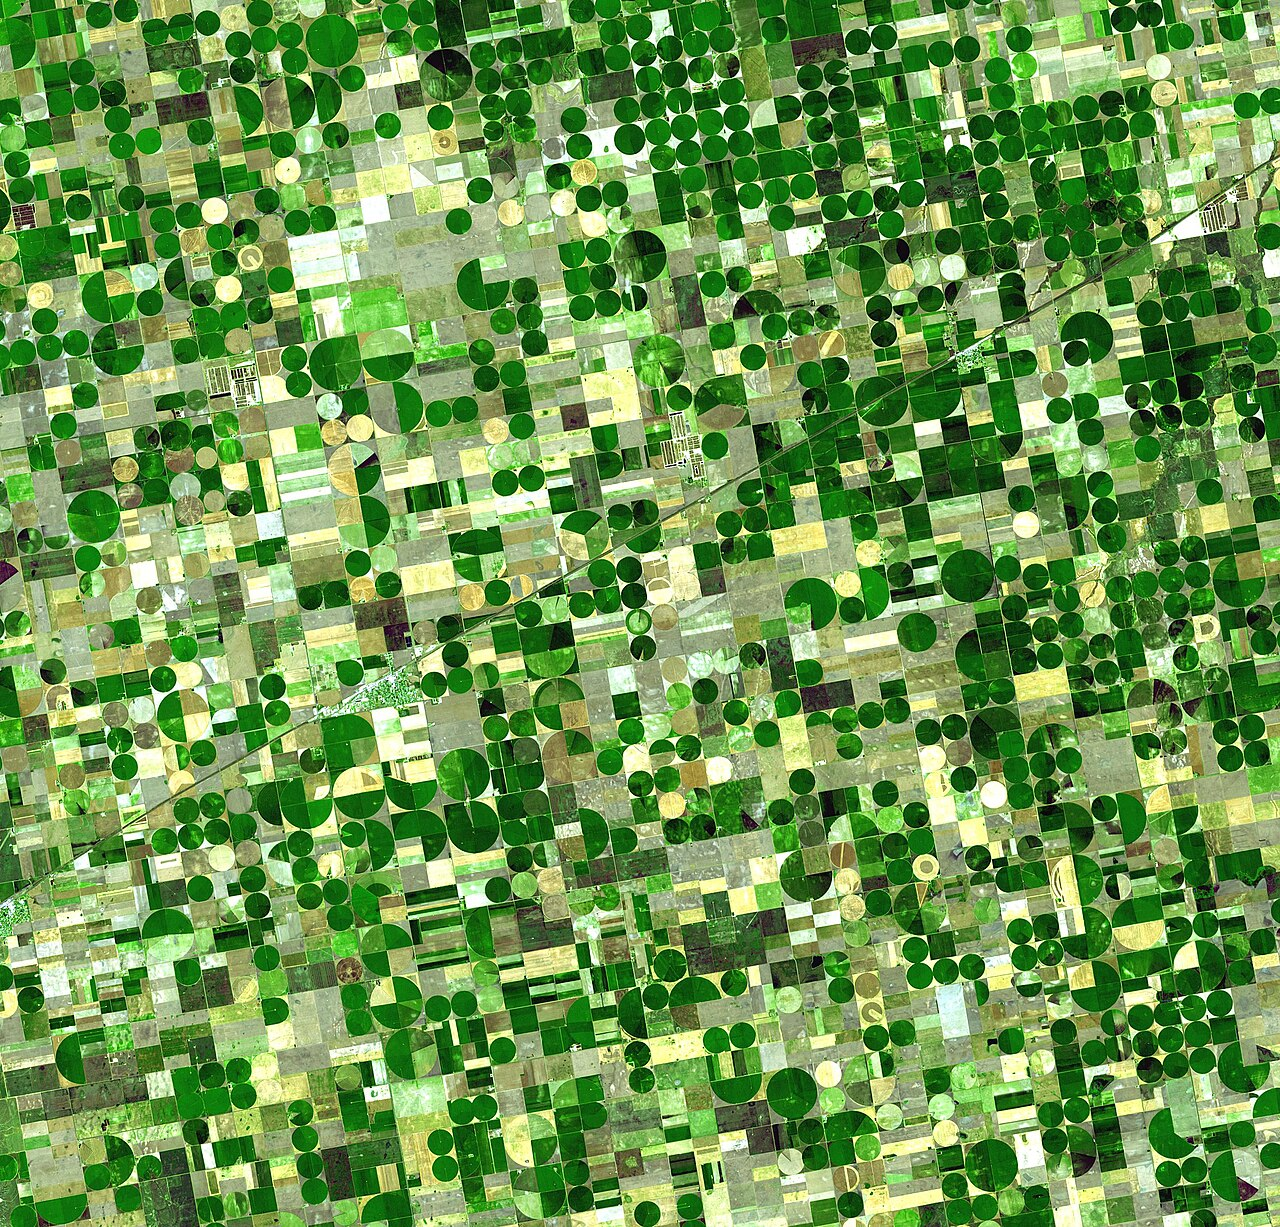
\includegraphics[width=0.5\linewidth]{images/book2/g10-nasa-kansas-center-pivot.jpg}

{\small Geïrrigeerde akkers bij Sublette, Kansas, gezien door het ASTER-instrument
van NASA's Terra-satelliet in juni 2001 (ongeveer \qty{37}{km} breed). Elke cirkel
is een akker die wordt besproeid door een lange sproeiarm die om zijn middelpunt
draait; de cirkels hebben een middellijn van \num{800} en \qty{1600}{m}. Beeld:
NASA (publiek domein).}
\end{omfigure}

Grondwater is vanuit de ruimte niet te zien, maar het kan wel worden gewogen: twee
satellieten die achter elkaar vliegen, voelen de kleine veranderingen in de
aantrekking van de Aarde die worden veroorzaakt door de massa water die onder hen
komt en gaat, en brengen in kaart waar de watervoorraad op het land van maand tot
maand stijgt en daalt.

\begin{omfigure}
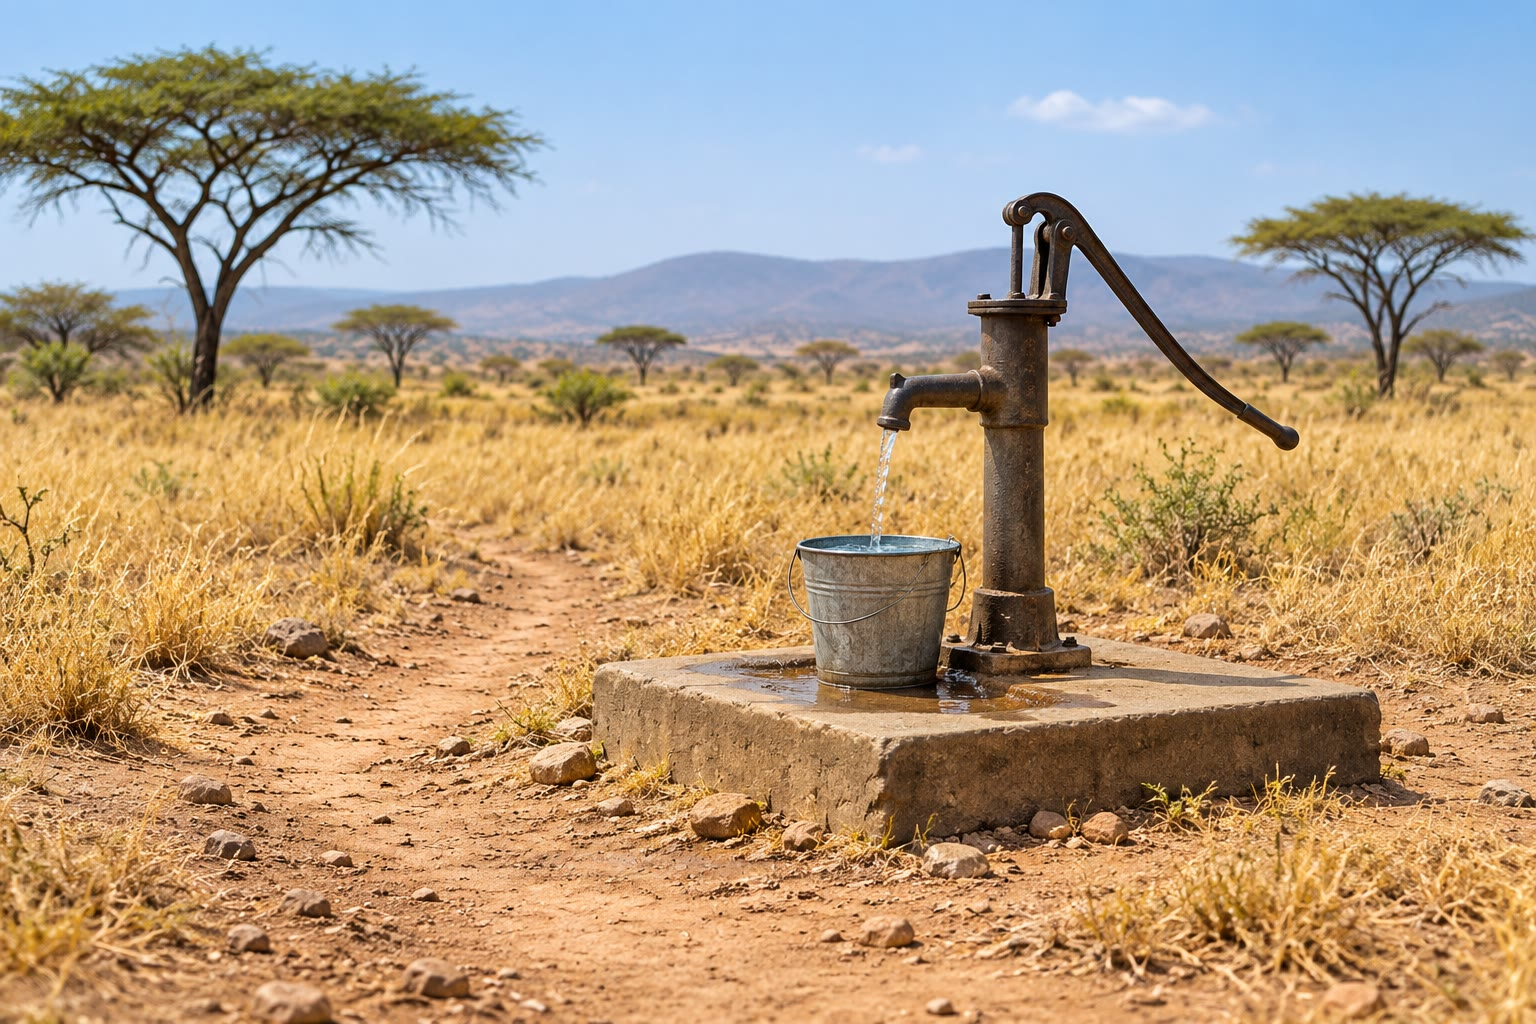
\includegraphics[width=0.55\linewidth]{images/book2/ai/g10-hand-pump-well.jpg}

{\small Een handpomp op een put in een droog landschap: het water dat hier wordt
opgepompt, komt uit de grond eronder, buiten het bereik van het droge seizoen.}
\end{omfigure}

\section{Overmatig gebruik als natuurkundig feit}

Het Aralmeer heeft geen uitstroom: het water van zijn twee rivieren, de Amu Darja
en de Syr Darja, verdwijnt alleen door verdamping. In 1960 besloeg het
\qty{68000}{km^2}, bevatte het \qty{1093}{km^3}, en bevatte zijn water \qty{10}{g}
zout per liter. Dat jaar nam de verdamping \qty{71.1}{km^3} weg, en bracht de regen
op het meer \qty{9.4}{km^3}: om zijn peil te behouden had het meer
$71.1 - 9.4 = \qty{61.7}{km^3}$ per jaar uit zijn rivieren nodig.
% ledger: gaybullaev:aral-1960, gaybullaev:aral-table

Vanaf de jaren 1960 werden de rivieren omgeleid om de woestijn te irrigeren, en
bereikte bijna niets van hun water het meer: in de jaren 1970 en 1980 vaak minder
dan \qty{2}{km^3} per jaar. De verdamping ging door, en het meer begon te
krimpen. De balans bepaalt hoe snel. De verdamping neemt een laag water weg
waarvan de dikte van het klimaat afhangt, hier ongeveer een meter per jaar
($71.1/68\,000 \approx \qty{0.00105}{km}$). Als de toevoer stopt, daalt het peil
elk jaar met ongeveer zoveel, min de regen. Naarmate het meer krimpt, krimpen ook
zijn oppervlakte en dus zijn verdamping, en vertraagt de daling; maar ze stopt
pas wanneer toevoer en verdamping weer in evenwicht zijn.
% ledger: gaybullaev:aral-table (values computed in figdata/grade-10/aral_sea.py)

\begin{omfigure}
\begin{tikzpicture}
\begin{axis}[omrecord, name=vol, width=0.46\linewidth, height=5.4cm, xmin=1955, xmax=2012, ymin=0, ymax=1200,
  xtick={1960,1980,2000}, xticklabel style={/pgf/number format/1000 sep={}}, scaled y ticks=false,
  ylabel={volume (\unit{km^3})}, xlabel={jaar}, tick label style={font=\small}, label style={font=\small},
  title={\small watervolume}]
\addplot[omDef, line width=1pt, mark=*, mark size=1.3pt] table[x=year, y=volume] {figdata/out/grade-10-aral_sea-record.dat};
\end{axis}
\begin{axis}[omrecord, at={(vol.east)}, anchor=west, xshift=1.4cm, width=0.46\linewidth, height=5.4cm,
  xmin=1955, xmax=2012, ymin=0, ymax=140, xtick={1960,1980,2000},
  xticklabel style={/pgf/number format/1000 sep={}},
  ylabel={zoutgehalte (\unit{g/L})}, xlabel={jaar}, tick label style={font=\small}, label style={font=\small},
  title={\small zoutgehalte}]
\addplot[omProp, line width=1pt, mark=*, mark size=1.3pt] table[x=year, y=salinity] {figdata/out/grade-10-aral_sea-record.dat};
\end{axis}
\end{tikzpicture}

{\small Het Aralmeer van 1960 tot 2010: het volume van zijn water daalde tot een
tiende, terwijl het zout dat de verdamping achterliet dertien keer geconcentreerder
werd. Gegevens: Gaybullaev en anderen (2012).}
\end{omfigure}
% ledger: gaybullaev:aral-table

Tegen 2010 bevatte het meer \qty{98}{km^3}, een tiende van zijn volume van 1960,
over \qty{14280}{km^2}; zijn zoutgehalte had \qty{130}{g/L} bereikt, veel zouter
dan de oceaan. Zijn peil was met meer dan \qty{20}{m} gedaald. Van de droge bodem
waait zout stof op. De oorzaak is niet verborgen: de toevoer van het meer werd
afgesneden, terwijl zijn verdamping dat niet werd.
% ledger: gaybullaev:aral-table, gaybullaev:aral-1960, micklin:aral, nasa:aral

\section{Oefeningen}

\begin{exercise}[$\star$]\label{exo:g10:freshwater-resources:1}
Definieer een \omterm{def:g10:freshwater-resources:stock}{voorraad}, een \omterm{def:g10:freshwater-resources:stock}{flux} en een \omterm{def:g10:freshwater-resources:residence-time}{verblijftijd}, en geef van elk de eenheden.
\end{exercise}

\begin{exercise}[$\star$]\label{exo:g10:freshwater-resources:2}
Uit de tabel van het water van de wereld: welk deel van al het water is zoet?
Welke delen van het zoete water zijn bevroren en ondergronds? Welk reservoir
bevat het minst?
\end{exercise}

\begin{exercise}[$\star$]\label{exo:g10:freshwater-resources:3}
Definieer \omterm{def:g10:freshwater-resources:renewable}{hernieuwbaar zoet water} en \omterm{def:g10:freshwater-resources:fossil-groundwater}{fossiel grondwater}. Waarom is het eerste een
\omterm{def:g10:freshwater-resources:stock}{flux} en het tweede een \omterm{def:g10:freshwater-resources:stock}{voorraad}?
\end{exercise}

\begin{exercise}[$\star$]\label{exo:g10:freshwater-resources:4}
Hoeveel keer meer water bevatten de zoetwatermeren van de wereld
(\num{91000}~\unit{km^3}) dan de rivieren (\num{2120}~\unit{km^3})?
\end{exercise}

\begin{exercise}[$\star$]\label{exo:g10:freshwater-resources:5}
Welk reservoir vernieuwt op de grafiek van de \omterm{def:g10:freshwater-resources:residence-time}{verblijftijden} zijn water het
snelst, en welk het traagst? Hoeveel keer langer blijft water in de oceaan dan
in de lucht?
\end{exercise}

\begin{exercise}[$\star\star$]\label{exo:g10:freshwater-resources:6}
De atmosfeer bevat \num{12700}~\unit{km^3} water. Bereken de \omterm{def:g10:freshwater-resources:residence-time}{verblijftijd} uit de
verdamping die erin komt (\num{413000} uit de oceaan en
\num{73000}~\unit{km^3} van het land per jaar), en ga na dat ze overeenkomt met
de \omterm{def:g10:freshwater-resources:residence-time}{verblijftijd} berekend uit de neerslag die eruit gaat.
\end{exercise}

\begin{exercise}[$\star\star$]\label{exo:g10:freshwater-resources:7}
De oceaan bevat \num{1335040} duizend~\unit{km^3} en verliest
\num{413} duizend~\unit{km^3} per jaar door verdamping. Bereken zijn
\omterm{def:g10:freshwater-resources:residence-time}{verblijftijd}. Waarom is ze dezelfde als je rekent met wat erin komt?
\end{exercise}

\begin{exercise}[$\star\star$]\label{exo:g10:freshwater-resources:8}
Schrijf met de \omterm{def:g10:freshwater-resources:stock}{fluxen} van de wereldwijde waterkringloop de balans van het land op:
wat erop valt, wat naar de lucht terugkeert, wat afstroomt. Welk deel van de regen
die op het land valt, keert terug naar de lucht?
\end{exercise}

\begin{exercise}[$\star\star$]\label{exo:g10:freshwater-resources:9}
De watervoerende laag van de High Plains verloor van ongeveer 1950 tot 2015
ongeveer \num{273.2} miljoen acre-voet water (\num{1}~acre-voet = \qty{1233.5}{m^3}).
Reken dit volume om naar \unit{km^3} en vergelijk het met het volume van het
Aralmeer in 1987 (\qty{345.6}{km^3}).
\end{exercise}

\begin{exercise}[$\star\star$]\label{exo:g10:freshwater-resources:10}
Het gemiddelde waterpeil van de watervoerende laag van de High Plains daalde van
ongeveer 1950 tot 2015 met \num{15.8} voet (\num{1}~voet = \qty{0.3048}{m}).
Hoeveel is dat in meter, en in centimeter per jaar?
\end{exercise}

\begin{exercise}[$\star\star$]\label{exo:g10:freshwater-resources:11}
Een watervoerende laag bevat \qty{2}{km^3} water en wordt aangevuld met
\qty{0.01}{km^3} per jaar. Wat is de \omterm{def:g10:freshwater-resources:residence-time}{verblijftijd} van het water? Putten pompen er
nu \qty{0.05}{km^3} per jaar uit. Stel dat de aanvulling doorgaat en dat de
putten nu de enige uitweg voor het water zijn: hoe lang zal het water dan
meegaan?
\end{exercise}

\begin{exercise}[$\star\star\star$]\label{exo:g10:freshwater-resources:12}
Bereken de \omterm{def:g10:freshwater-resources:residence-time}{verblijftijd} van het water van het Aralmeer in 1960
(\qty{1093}{km^3}, verdamping \qty{71.1}{km^3} per jaar) en in 2010
(\qty{98.1}{km^3}, verdamping \qty{11.4}{km^3} per jaar). Waarom nam de
verdamping af?
\end{exercise}

\begin{exercise}[$\star\star\star$]\label{exo:g10:freshwater-resources:13}
Een meer zonder uitstroom beslaat \qty{100}{km^2}. De verdamping neemt elk jaar
\qty{1.2}{m} water van het oppervlak weg, en de regen voegt \qty{0.2}{m} toe.
\begin{enumerate}
  \item Welke toevoer, in \unit{km^3} per jaar, houdt het peil constant?
  \item De toevoer wordt gehalveerd. Hoeveel daalt het peil in het eerste
        jaar?
  \item Waarom vertraagt de daling in de jaren daarna?
\end{enumerate}
\end{exercise}

\begin{exercise}[$\star\star\star$]\label{exo:g10:freshwater-resources:14}
In een woestijn vult regen een watervoerende laag aan met \qty{1}{mm} water per
jaar. De laag is \qty{100}{m} dik en water vult \qty{20}{\percent} van haar
volume. Hoe lang zou de aanvulling erover doen om haar te vullen? Vergelijk met
de ouderdom van het diepe water van de watervoerende laag onder de Sahara.
\end{exercise}

\begin{exercise}[$\star\star\star$]\label{exo:g10:freshwater-resources:15}
De watervoerende laag van de High Plains beslaat ongeveer \qty{453000}{km^2} en
had tegen 2015 ongeveer \qty{337}{km^3} water verloren. Welke waterdikte, verspreid
over de hele laag, is dat? Het waterpeil daalde gemiddeld met \qty{4.8}{m}.
Waarom is de daling van het waterpeil groter dan de verloren waterdikte?
\end{exercise}

\section{Probleem: de balans van het Aralmeer}

\begin{problem}[{Weekendprobleem --- hoe snel verdwijnt een meer?}]
\label{pb:g10:freshwater-resources:1}
% ledger: gaybullaev:aral-table, gaybullaev:aral-1960, micklin:aral (values computed in figdata/grade-10/aral_sea.py)
De tabel geeft de balans van het Aralmeer voor vier jaren (volumes in
\unit{km^3}, zoutgehalte in gram zout per liter). In 1960 besloeg het meer
\qty{68000}{km^2}.
\begin{center}
\small
\begin{tabular}{|c|c|c|c|c|c|}
\hline
jaar & rivierinstroom & regen op het meer & verdamping & volume & zoutgehalte \\ \hline
1960 & 42.0 & 9.4 & 71.1 & 1093.0 & 10.0 \\ \hline
1984 & 0.3 & 3.5 & 47.9 & 502.7 & 21.9 \\ \hline
1987 & 1.0 & 6.2 & 36.8 & 345.6 & 25.0 \\ \hline
1989 & 3.1 & 5.3 & 35.3 & 327.2 & 30.0 \\ \hline
\end{tabular}

{\small Gegevens: Gaybullaev en anderen (2012).}
\end{center}

\medskip
\noindent\textbf{Deel I --- Het meer in 1960.}
\begin{enumerate}
  \item Wat was de gemiddelde diepte van het meer in 1960?
  \item Druk zijn volume uit in kubieke meter.
  \item Welke massa zout bevatte het, in ton?
  \item Wat was de \omterm{def:g10:freshwater-resources:residence-time}{verblijftijd} van zijn water, gerekend met de verdamping?
  \item Waarom kan een meer zonder uitstroom alleen water verliezen door
        verdamping (en insijpeling)?
\end{enumerate}

\medskip
\noindent\textbf{Deel II --- Wat het meer nodig heeft.}
\begin{enumerate}[resume]
  \item Welke waterdikte nam de verdamping in 1960 van het meer weg, in
        meter?
  \item Welke dikte voegde de regen toe?
  \item Welke rivierinstroom zou verdamping en regen precies in evenwicht hebben
        gehouden?
  \item De twee rivieren voeren gemiddeld ongeveer \qty{79}{km^3} en
        \qty{37}{km^3} per jaar uit de bergen af. Welk deel daarvan zou het
        meer nodig hebben?
\end{enumerate}

\medskip
\noindent\textbf{Deel III --- Het meer aan het eind van de jaren 1980.}
\begin{enumerate}[resume]
  \item Schrijf de balans van 1987 op: inkomsten, uitgaven, nettoverandering.
  \item Tussen 1984 en 1989 daalde het volume van \qty{502.7}{km^3} naar
        \qty{327.2}{km^3}. Wat was de gemiddelde daling per jaar? Vergelijk met
        de balans van 1987.
  \item Neem aan dat een vierkante kilometer meer evenveel water door verdamping
        verliest als in 1960. Wat was de oppervlakte van het meer in 1987?
  \item Welk deel van zijn oppervlakte van 1960 is dat?
  \item Waarom was de verdamping gedaald van \qty{71.1}{km^3} naar
        \qty{36.8}{km^3}?
  \item Welk deel van zijn volume van 1960 bevatte het meer in 1987 nog?
\end{enumerate}

\medskip
\noindent\textbf{Deel IV --- Het zout en het peil.}
\begin{enumerate}[resume]
  \item Als al het zout van 1960 in het water was gebleven, wat zou het
        zoutgehalte in 1987 dan zijn geweest?
  \item De tabel geeft \qty{25.0}{g/L}. Wat doet het verschil vermoeden?
  \item Hoeveel zou het peil elk jaar dalen zonder enige toevoer en zonder
        enige regen?
  \item Hoeveel voegden de rivieren en de regen in 1987 toe, als dikte over de
        oppervlakte van vraag 12?
  \item Hoeveel daalde het peil van het Aralmeer in 1987?
\end{enumerate}
\end{problem}
